\documentclass[a4paper,11pt,cours]{nsi} % COMPILE WITH DRAFT
\geometry{margin=2cm}
\usepackage{hyperref}

\begin{document}

\setcounter{chapter}{5} % 1 de moins que le num de chapitre



\chapter{Suites arithmétiques et\\ géométriques}


\setlength{\columnseprule}{0.5pt}
\setlength{\columnsep}{1cm}



\section{Deux exemples d'étude de suites}
\begin{exercice}[ ]
	En 2020, un village U comptait 800 habitants mais chaque année il perd 5 habitants au profit d’un village V qui comptait 580 habitants en 2020.\\[.5em]
	\textbf{En quelle année, la population du village V dépassera-telle celle du village U ?}
\end{exercice}

\subsection*{Modélisation de la situation avec des suites}
\begin{definition}[ ]
	Une suite $(u_n)$ est dite \textbf{arithmétique} s'il existe un nombre réel $r$ tel que pour tout entier $n$ on a $u_{n+1}=u_n+r$ .\\
	Le nombre $r$ est appelé \textbf{raison} de la suite $(u_n)$.\\[.5em]
	\textbf{Schéma général :}
	\vspace{2cm}
\end{definition}
\carreauxseyes{16.8}{7.2}


\subsection*{Procédure 1 : Utilisation des formes explicites des deux suites}
\begin{propriete}[ ]
	Si $(u_n)$ est une suite \textbf{arithmétique} de raison $r$, alors pour tous entiers naturels $n$ et $m$ :
	\begin{enumerate}[label=\textbullet]
		\item 	$u_n = u_0+n\times r$ \hspace{.5cm}(forme explicite)
		\item 	$u_n=u_m+(n-m)r$	
    \end{enumerate}
  
\end{propriete}
\carreauxseyes{16.8}{8.8}

\subsection*{Procédure 2 : Utilisation des représentations graphiques des deux suites}
\begin{propriete}[ ]
	Si $(u_n)$ est une suite \textbf{arithmétique} de raison $r$, alors, dans un repère, les points de coordonnées $(n\ ;u_n)$ sont alignés.
\end{propriete}
\petitscarreaux{17}{8}



\begin{multicols}{2}
	\subsection*{Procédure 3 : Utilisation d'un tableur}
	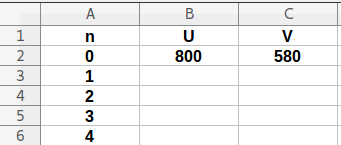
\includegraphics[width=8cm]{tableur1}\\
	
	\vspace{3cm}
	
	\subsection*{Procédure 4 : Utilisation d'un algorithme}
	\begin{pyc}
        \begin{minted}{python}
u = ...
v = ...
n = ...

while u ... v :
    u = ...
    v = ...
    n = ...

print(...)
        \end{minted}
    \end{pyc}
\end{multicols}

\carreauxseyes{16.8}{6.4}
\vspace{.5cm}

\begin{exercice}[ ]
	Mathieu a placé 4000 € sur un compte qui rapporte 2 \% d’intérêts chaque année.\\ Julie a placé 3500 € sur un compte qui rapporte 3 \% d’intérêts chaque année.\\[.5em]
	\textbf{Au bout de combien d’années, Julie disposera-telle de plus d’argent que Mathieu ?}
\end{exercice}

\subsection*{Modélisation de la situation avec des suites}
\begin{definition}[ ]
	Une suite $(u_n)$ est dite \textbf{géométrique} s'il existe un nombre réel $q$ tel que pour tout entier $n$ on a $u_{n+1}=q \times u_n$ .\\
	Le nombre $q$ est appelé \textbf{raison} de la suite $(u_n)$.\\[.5em]
	\textbf{Schéma général :}
	\vspace{2cm}
\end{definition}
\newpage
\carreauxseyes{16.8}{6.4}\\



\subsection*{Procédure 1 : Utilisation des formes explicites des deux suites}
\begin{propriete}[ ]
	Si $(u_n)$ est une suite \textbf{géométrique} de raison $q\neq 0$, alors pour tous entiers naturels $n$ et $m$ :
	\begin{enumerate}[label=\textbullet]
		\item 	$u_n = u_0\times q^n $  \hspace{.5cm}(forme explicite)
		\item 	$u_n=u_m\times q^{n-m}$	
	\end{enumerate}
\end{propriete}
\carreauxseyes{16.8}{5.6}

\begin{multicols}{2}
	\subsection*{Procédure 2 : Utilisation d'un tableur}
	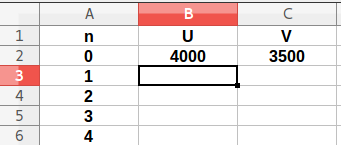
\includegraphics[width=8cm]{tableur2}\\
	
	\vspace{2cm}
	
	\subsection*{Procédure 3 : Utilisation d'un algorithme}
	\carreauxseyes{8}{5.6}
\end{multicols}

\section{Sens de variation d'une suite arithmétique ou géométrique}
\begin{propriete}
	Soit $u$ une suite arithmétique de raison $r$.
	\begin{enumerate}[label=\textbullet]
		\item {\boldmath\textbf{si $r>0$ alors $u$ est croissante.}}
		\item {\boldmath\textbf{si $r<0$ alors $u$ est décroissante.}}
		\item {\boldmath\textbf{si $r=0$ alors $u$ est constante.}}
	\end{enumerate}
\end{propriete}
\begin{demonstration}
	\carreauxseyes{16}{8}
\end{demonstration}

\begin{exemple}
	\begin{minipage}{9.5cm}
			Soit la suite $\alpha$ définie par
		$$\left\{
		\begin{array}{llll}
			\alpha_0 & = & 4 & \\
			\alpha_{n+1} & = & \alpha_n-\dfrac{1}{2} & \text{pour tout } n\in\N\\
		\end{array}
		\right. $$
		C'est une suite arithmétique de raison $-\dfrac{1}{2}$, c'est donc une suite décroissante.
	\end{minipage}
	\begin{minipage}{7cm}
		\begin{center}
			\def\xmin{-1} \def\ymin{-1}\def\xmax{7}\def\ymax{5}
			\begin{tikzpicture}[scale=.8]
				\clip (\xmin,\ymin) rectangle (\xmax,\ymax);
				\draw[fill = white] (\xmin,\ymin) rectangle (\xmax,\ymax);
				\repereal{\xmin}{\ymin}{\xmax}{\ymax}
				\draw 	(0,4)	\ball node[below right]{$A_0$}		(1,3.5)	\ball node[below right]{$A_1$}
				(2,3)	\ball node[below right]{$A_2$} 		(3,2.5)	\ball node[below right]{$A_3$}
				(4,2)\ball node[below right]{$A_4$} 		(5,1.5)	\ball node[below right]{$A_5$}
				(6,1)	\ball node[below right]{$A_6$};
			\end{tikzpicture}
		\end{center}
	\end{minipage}
	
\end{exemple}

\begin{propriete}
	Soit $u$ une suite géométrique de raison $q$.
	\begin{enumerate}[label=\textbullet]
		\item 	Si $q<0$ la suite n'est ni croissante ni décroissante.
		\item 	Si $q=0$ la suite est nulle à partir de $u_1$.
		\item 	Si $q=1$ la suite est constante.
	\end{enumerate}
	\begin{multicols}{2}
		\begin{enumerate}[label=\textbullet]
			\item 	Si $u_0>0$ alors 	\begin{itemize}
				\item 	Si $q>1$ la suite est croissante.
				\item 	Si $0<q<1$ la suite est décroissante.
			\end{itemize}
			\item 	Si $u_0<0$ alors 	\begin{itemize}
				\item 	Si $q>1$ la suite est décroissante.
				\item 	Si $0<q<1$ la suite est croissante.
			\end{itemize}		
		\end{enumerate}
	\end{multicols}
\end{propriete}	

\begin{demonstration}
	\carreauxseyes{16}{8.8}
\end{demonstration}	

\begin{exemple}[s]
	\begin{minipage}{9.3cm}
		La suite $u$ définie par
		$$\left\{\begin{array}{llll}
			u_0 & = &6 & \\
			u_{n+1} & = & \dfrac{2}{3}u_n & \text{pour tout } n\in\N\\
		\end{array}
		\right. $$
		est une suite géométrique de raison $q=\dfrac{2}{3}$.\\[.5em]
		Comme $u_0>0$ et que $0<q<1$, elle est décroissante.
	\end{minipage}
	\begin{minipage}{7cm}
		\begin{center}
			\def\xmin{-1} \def\ymin{-1}\def\xmax{7}\def\ymax{7}
			\begin{tikzpicture}[scale=.6]
				\clip (\xmin,\ymin) rectangle (\xmax,\ymax);
				\draw[fill = white] (\xmin,\ymin) rectangle (\xmax,\ymax);
				\repereal{\xmin}{\ymin}{\xmax}{\ymax}
				\draw 	(0,6)	\ball node[below right]{$A_0$}		(1,4)	\ball node[above right]{$A_1$}
				(2,2.66666)	\ball node[above right]{$A_2$} 		(3,1.77777)	\ball node[above right]{$A_3$}
				(4,1.185185)\ball node[above right]{$A_4$} 		(5,0.7901423)	\ball node[above right]{$A_5$}
				(6,0.526748)	\ball node[above right]{$A_6$};
			\end{tikzpicture}
		\end{center}
	\end{minipage}
	
	\vspace{.5cm}
	
	\begin{minipage}{9.3cm}
		La suite $v$ définie par
		$$\left\{\begin{array}{llll}
			v_0 & = &1 & \\
			v_{n+1} & = & 1,34\ v_n & \text{pour tout } n\in\N\\
		\end{array}
		\right. $$
		est une suite géométrique de raison $q=1,34$.\\[.5em] 
		Comme $u_0>0$ et que $q<1$, elle est croissante.
	\end{minipage}
	\begin{minipage}{7cm}
		\begin{center}
			\def\xmin{-1} \def\ymin{-1}\def\xmax{7}\def\ymax{7}
			\begin{tikzpicture}[scale=.6]
				\clip (\xmin,\ymin) rectangle (\xmax,\ymax);
				\draw[fill = white] (\xmin,\ymin) rectangle (\xmax,\ymax);
				\repereal{\xmin}{\ymin}{\xmax}{\ymax}
				\draw 	(0,1)	\ball node[below right]{$A_0$}		(1,1.34)	\ball node[below right]{$A_1$}
				(2,1.7956)	\ball node[below right]{$A_2$} 		(3,2.406)	\ball node[below right]{$A_3$}
				(4,3.224)\ball node[below right]{$A_4$} 		(5,4.32)	\ball node[below right]{$A_5$}
				(6,5.789)	\ball node[below right]{$A_6$};
			\end{tikzpicture}
		\end{center}
	\end{minipage}
	
\end{exemple}

\section{Somme de termes consécutifs d'une suite arithmétique ou géométrique}
\subsection*{Sommes des termes d'une suite arithmétique}
\begin{propriete}[]
	Pour tout entier $n\geqslant1, \quad 0+1+2+3+\ldots+n = \dfrac{n(n+1)}{2} $\\
	\begin{minipage}{2cm}
		On note :
	\end{minipage}
	\begin{minipage}{6cm}
		$$\quad\sum_{k=0}^n k = \dfrac{n(n+1)}{2}.$$
	\end{minipage} 
\end{propriete}
\begin{demonstration}
	\carreauxseyes{16}{10.4}\\
	Démonstration en vidéo : \href{https://youtu.be/hHySWepnHwY}{https://youtu.be/hHySWepnHwY}
\end{demonstration}	

\begin{encadrecolore}{Histoire}{UGLiBlue}
	\dleft{2cm}{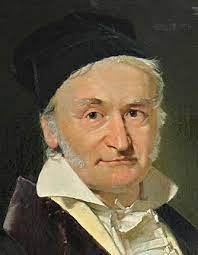
\includegraphics[width=2cm]{Gauss}}{
		Une anecdote raconte que le jeune Carl Friedrich Gauss (1777 - 1855), alors âgé de 10 ans a utilisé cette astuce pour effectuer très rapidement et avant tous ses camarades un calcul donné par son instituteur. Il s'agissait de calculer la somme $1+2+3+...+100$.\\
		Pour en savoir plus : \href{https://youtu.be/pvKLXuueQTI}{https://youtu.be/pvKLXuueQTI}}
        
\end{encadrecolore}

\newpage

\begin{propriete}[ : Somme des termes d'une suite arithmétique]
	Soit $(u_n)$ une suite arithmétique de raison $r$ et de premier terme $u_0$.\\
	Soient $n$ et $p $ deux entiers naturels, avec $n<p$.
	\begin{enumerate}[label=\textbullet]
		\item La somme des $n+1$ premiers termes de la suite $u_n$ est égale à :
		$$u_0+u_1+u_2+...u_{n-1}+u_n=(n+1)\dfrac{u_0+u_n}{2}$$
		\item La somme des termes d'indice $p$ à $n$ est égale à :
		$$u_p+u_{p+1}+...+u_n=(n-p+1)\dfrac{u_p+u_n}{2}$$
	\end{enumerate}
\end{propriete}

\begin{demonstration}
	\carreauxseyes{16}{12}
\end{demonstration}

\subsection*{Somme des termes d'une suite géométrique}

\begin{propriete}
	Pour tout réel $q\neq 1$ et pour tout entier $n\geqslant 1$, on a :
	$\quad 1+q+q^2+\ldots+q^n=\dfrac{1-q^{n+1}}{1-q}.$
	\begin{minipage}{2cm}
		On note :
	\end{minipage}
	\begin{minipage}{6cm}
		$$\sum_{k=0}^n q^k = \frac{1-q^{n+1}}{1-q}.$$
	\end{minipage}
\end{propriete}

\begin{demonstration}
	%\carreauxseyes{16}{12}\\
	Soient $n\in\N^*$ et $q\in\R\setminus \left\{1\right\}$.\\
	On note: $S_n=1+q+q^2+...+q^{n-2}+q^{n-1}+q^n$.
	\begin{tabbing}
		On a : $\qquad$ \= $q \times S_n=q+q^2+q^3+...+q^{n-1}+q^n+q^{n+1}$\\[.5em]
		D'où \> $S_n-qS_n = 1 + q-q + q^2-q^2 + ... + q^n-q^n-q^{n+1}$\\[.5em]
			\>	$1\times S_n -qS_n=1-q^{n+1}$\\[.5em]
			\>	$(1-q) S_n=1-q^{n+1}$\\[.5em]
		Ainsi	\>	$S_n=\dfrac{1-q^{n+1}}{1-q} \qquad$ en divisant par $1-q$ car $q\neq 1$
	\end{tabbing}
\end{demonstration}

\begin{propriete}[ : Somme des termes d'une suite géométrique]
	Soit $(u_n)$ une suite géométrique de raison $q\neq 1$ et de premier terme $u_0$.\\
	Soient $n$ et $p $ deux entiers naturels, avec $n<p$.
	\begin{enumerate}[label=\textbullet]
		\item La somme des $n+1$ premiers termes de la suite $u_n$ est égale à :
		$$u_0+u_1+u_2+...u_{n-1}+u_n=u_0\times \dfrac{1-q^{n+1}}{1-q}$$
		\item La somme des termes d'indice $p$ à $n$ est égale à :
		$$u_p+u_{p+1}+...+u_n\times \dfrac{1-q^{n-p+1}}{1-q}$$
	\end{enumerate}
\end{propriete}

\begin{demonstration}
	\carreauxseyes{16}{10.4}
\end{demonstration}

\begin{exemple}[s]
	\begin{enumerate}
		\item 	Calculer $\quad S_1=1+2+3+...+75$.
		\item 	Calculer $\quad S_2=1+\dfrac{1}{3}+\left(\dfrac{1}{3}\right)^2+...+\left(\dfrac{1}{3}\right)^9$.
		\item 	La suite $(u_n)$ est arithmétique avec $u_3=3$ et $u_9=15$.\\
		Calculer $u_3+u_4+...+u_9$
		\item 	La suite $(v_n)$ est géométrique de raison $q=-2$ et de premier terme $v_0=3$.\\
		Calculer la somme des dix premiers termes de la suite $(v_n)$.
	\end{enumerate}
\end{exemple}
\carreauxseyes{16.8}{12}\\


\begin{exercice}[ ]
	Alice a deux propositions de salaires lors de son arrivée dans une entreprise le 1$^{\text{er}}$ janvier 2023 :
	\begin{enumerate}[label=\textbullet]
		\item 	\textbf{Proposition 1 :} Elle commence avec un salaire de 2000 € mensuel la première année et son salaire mensuel augmente chaque année de 115 €.
		\item 	\textbf{Proposition 2 :} Elle commence avec un salaire de 2000 € mensuel la première année et son salaire mensuel augmente chaque année de 5\%.
	\end{enumerate}
	Afin de se constituer un pécule pour faire le tour du monde en 2033, Alice souhaite mettre de côté \textbf{UN} salaire mensuel par an jusqu'à son départ.\\[.5em]
	Quelle proposition lui conseillez-vous de choisir ?
\end{exercice}
%\carreauxseyes{16.8}{18.4}
\end{document}
